\chapter{Concetti teorici}
Nell'approccio all'algoritmica e, in generale, alla programmazione, ci si concentra sempre sulla ricerca dell'algoritmo ottimo per la risoluzione di un problema. 
La Teoria della Complessità assume che l'esecutore della soluzione sia uno. 
Soprattutto, quest'ultima si concentra sul numero di operazioni necessarie alla risoluzione il problema dato. 
Tuttavia, sfruttando il concetto di parallelismo, è possibile ridurre il tempo effettivo di esecuzione, proprio in termini di secondi o sotto suoi multipli, nella risoluzione di un problema. 
Bisogna sin da subito notare che il parallelismo permette di eseguire una soluzione più velocemente, non di effettuare meno operazioni. Anzi, vedremo che, per sfruttare il parallelismo, saranno sovente richieste addirittura più operazioni.

\section{Parallelismo}
Il parallelismo consente di affrontare simultaneamente i sottoproblemi più piccoli di un problema. Ciò avviene introducendo più esecutori paralleli. 
Il parallelismo è un concetto che esiste anche solo teoricamente: un problema può essere analizzato in un ambiente teorico parallelo in via totalmente teorica, permettendo la valutazione di un algoritmo parallelo e il suo confronto con altre soluzioni prima di spostarsi su macchine reali.
Detto questo, esistono tre tipi di parallelismo:
\begin{itemize}
  \item \keyword{Parallelismo temporale}, anche chiamato pipeline (in italiano, catena di montaggio): operazioni diverse sullo stesso flusso di oggetti vengono eseguite da esecutori diversi, contemporaneamente. Il prodotto di una fase è usato come punto di partenza per la fase successiva;
  \item Parallelismo spaziale: la stessa operazione viene eseguita più volte, contemporaneamente, su più flussi di oggetti;
  \item Parallelismo asincrono: opreazioni diverse su flussi di oggetti diversi vengono eseguiti da esecutori diversi.
\end{itemize}

In termini di calcolatori classici, un processore completo (CPU) è composto da una \textit{control unit} (CU), che decodifica le operazioni i.e. moltiplicazioni, somme, etc. scomponendo queste ultime in istruzioni elementari, ed una ALU, che esegue tali istruzioni elementari. 
Una CU decodifica uno \textit{stream} di istruzioni, mentre una ALU gestisce uno \textit{stream} di dati. Possiamo implementari tutti i tre tipi di parallelismo mediante un insieme di CPU e ALU.
Il parallelismo temporale può essere implementato con una sola CU e più ALU, oppure con una sola ALU che abbia capacità di pipelining. Il parallelismo spaziale può essere implementato mediante una sola CU e tante ALU. Il parallelismo asincrono può essere implementato con più CPU. 
Sebbene quelle descritte non siano le uniche implementazioni possibili, esse sono sicuramente quelle minimali, ovvero quelle configurazioni di CPU e ALU strettamente necessarie per implementare il particolare tipo di parallelismo.

\subsection{Tassonomia di Flynn}
La tassonomia di Flynn è un modello di classificazione delle architetture dei calcolatori paralleli, introdotto da Michael J. Flynn nel 1966. Flynn ha proposto una classificazione basata su due concetti fondamentali: il flusso di istruzioni (Instruction Stream) e il flusso di dati (Data Stream). Ogni architettura viene classificata in base al numero di flussi di istruzioni e di dati che può gestire simultaneamente.

\begin{figure}[h]
\centering
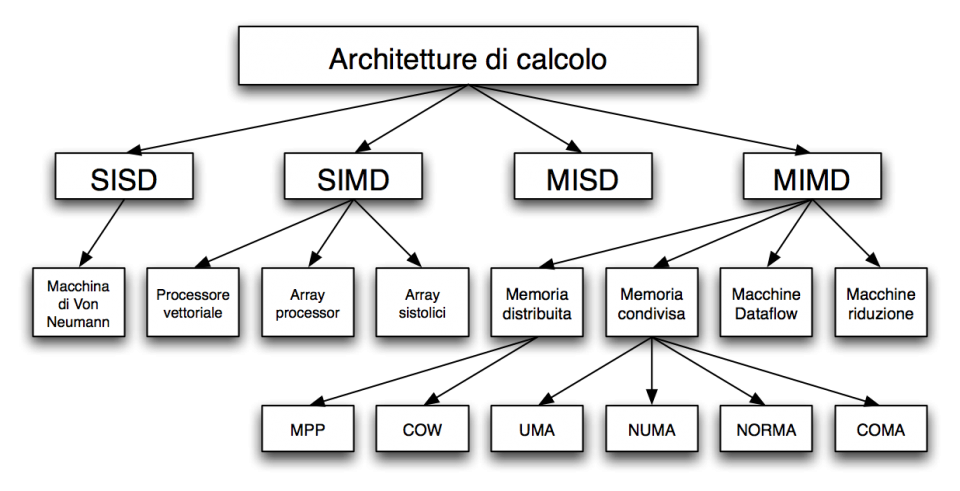
\includegraphics[width=0.5\textwidth]{../_files/_images/flynn-taxonomy.png}
\caption{La tassonomia di Flynn.}
\label{fig:flynn-taxonomy}
\end{figure}

\begin{note}{}
Nell'articolo in cui viene presentata la tassonomia, Flynn parla di Instruction stream, non di singola istruzione, e di Data stream, non di singolo dato. In questo contesto, la famiglia MISD assume senso: su un singolo stream di dati, vengono applicati tanti stream di istruzioni, intese come istruzioni aritmetiche. Pertanto, una macchina MISD prevede una singola CU ma con un ALU con capacità pipelining.
\end{note}

Sebbene la tassonomia di Flynn sia a fondamento della classificazione dei calcolatori, nel tempo si è passati sempre di più ad architetture ibride ed eterogenee. Si parla di \keyword{architettura ibrida} quando presenta più livelli di parallelismo, in cui i livelli appartengono a famiglie distinte di calcolatori parallali secondo la tassonomia di Flynn.
Si parla di \keyword{architettura eterogenea} quando, allo stesso livello architetturale, essa è composta da calcolatori appartenenti a famiglie diverse della tassonomia. Ad esempio un qualsiasi computer odierno è dotato di una CPU e di una GPU, che, pur essendo calcolatori di natura molto diversa, collaborano al primo livello dell'architettura.
Quest'ultimo è anche un esempio di architettura ibrida: una CPU è composta da vari core indipendenti collegati alla stessa memoria (MIMD-SM) e, all'interno di ciascun core, sono presenti unità di calcolo con capacità di pipelining (MISD).
Con il tempo, la tassonomia di Flynn è stata sottoposta all'aggiunta di nuove sottoclassi. Ad esempio, nella famiglia MIMD Shared Memory, si sono sviluppate due sottoclassi: SymmetricMultiProcessor (SMP) e ASymmetricMultiProcessor (ASMP).
In un SMP, i core sono uguali tra loro, mentre in un ASMP vi sono core di diversi tipi. Nei sistemi ASMP, i processi vengono distribuiti ai core in base a dipendenza e tipologia.

\subsection{Calcolo del costo}
Introduciamo al calcolo del costo di un algoritmo parallelo mediante un'algoritmo molto semplice: la somma di $n$ numeri.

La somma di $n$ numeri è calcolata mediante un'assegnazione iniziale e $n-1$ somme. Poiché il costo di un'assegnazione è considerato nullo (consideriamo operazione un'operazione aritmetica tra interi o tra floating point), il costo computazionale di questo problema è
$$T(n)= n-1$$
Avendo a disposizione un calcolatore MIMD Distributed Memory, in cui ogni processore si trova su un nodo separato e pertanto ha memoria privata, con $4$ nodi, è possibile adottare tre differenti strategie per ridurre il tempo effettivo di elaborazione.
Per prima cosa, possiamo distribuire gli $n$ addendi tra i $4$ nodi, cosicchè ciascun nodo avrà $\frac{n}{4}$ addendi. Se $n\not\equiv_{4}0$, allora qualche nodo avrà meno addendi rispetto agli altri, anche ridistribuendo equamente il resto. 
Completata la distribuzione, ciascun nodo calcola la propria somma parziale. 

\begin{note}{}
  Si noti che il numero di operazioni effettuate è $(\frac{n}{4} - 1)\cdot 4$, a cui bisogna, però, aggiungere il costo di distribuzione dei dati per calcolare in modo corretto il tempo di esecuzione. Tali operazioni vengono effettuate **contemporaneamente**.
\end{note}

A questo punto, dobbiamo elaborare una strategia per calcolare la somma totale a partire da quelle parziali. È necessario lo scambio dei dati (\keyword{message passing}) tra i nodi:
\begin{itemize}
  \item (Strategia 1) ciascun nodo invia la propria somma parziale ad un unico nodo prestabilito;
  \item (Strategia 2) i nodi vengono suddivisi in coppie, in cui il primo nodo della coppia invia all'altro la propria somma parziale. Il nodo ricevente della coppia potrà calcolare la somma delle somme parziali. Una volta calcolate le somme parziali di secondo livello, i nodi riceventi formeranno una coppia ed uno solo dei due riceverà la somma dell'altro. Infine, tale nodo potrà calcolare la somma totale;
  \item (Strategia 3) come la seconda strategia, ma entrambi i nodi della coppia inviano e ricevono, in modo tale che la somma totale sia infine calcolata da tutti i nodi.
\end{itemize}
Nella prima strategia, vengono effettuate $3$ operazioni (un'assegnazione e tre addizioni), in modo sequenziale. Nella seconda strategia, vengono effettuate $2$ operazioni al primo passo (due assegnazioni e due addizioni) e $1$ al secondo passo (un'assegnazione e un'addizione). 
Le $2$ operazioni del primo passo avvengono in parallelo, mentre l'unica operazione del secondo passo avviene in modo sequenziale.
Nella terza strategia, vengono effettuate $4$ operazioni al primo passo, $4$ al secondo e $4$ al terzo. Tutte le operazioni avvengono in parallelo.

\begin{note}
  La terza strategia potrebbe un'inutile complicazione della seconda: perché effettuare più calcoli solo per avere il risultato finale in tutti i nodi? Cerchiamo di rispondere enumerando i vantaggi di questo approccio:
  \begin{enumerate}
    \item poiché i nodi devono essere sincronizzati, non c'è alcun vantaggio nel far riposare un nodo durante il calcolo, a meno che non sia strettamente necessario liberare quanto prima i nodi. Insomma, facendo lavorare di più tutti i nodi, si sfrutta meglio la potenza computazionale a disposizione;
    \item avere il risultato finale in tutti i nodi può essere utile se si vuole utilizzare tale risultato su ciascuno di quei nodi;
  \end{enumerate}
\end{note}

\subsection{Speedup, overhead}
In generale, il tempo di esecuzione di un algoritmo è
$$T^{\text{time}}(n)=T(n)\cdot t_{\text{calc}}$$
dove $t_{\text{calc}}$ indica il tempo, in secondi o sottomultipli, per l'elaborazione di una floating point operation (\textit{flop}).
Potendo però sfruttare il parallelismo, $T^{\text{time}}$ dipende non più dal numero di operazioni bensì dal numero di passi temporali impiegati. 
Idealmente, si avrebbe
$$T^{\text{time}}(n)=\frac{T(n)}{p}\cdot t_{\text{calc}}$$
dove $p$ è il numero di processori a disposizione.

Ritorniamo all'esempio della somma di $n$ numeri ed osserviamo come varia il tempo di esecuzione dell'algoritmo al variare del numero di processori.
$$T^{\text{time}}_{p}(16)=\begin{cases}
15 &p=1 \\
8=7+1 &p=2 \\
5=3+2 &p=4 \\
4=1+3 &p=8 \\
4=0+4 &p=16 \\
5=0+5 &p=32 \\
\vdots
\end{cases}$$
da cui ricaviamo che
$$T^{\text{time}}(p):=T^{\text{time}}_{p}(n)=\left[\left(\left\lceil   \frac{n}{p}\right\rceil-1\right) + \log_2(p)\right]t_{\text{calc}} $$

\begin{definition}{Speedup}
Il rapporto $S(p) =\frac{T(1)}{T(p)}$ è chiamato \keyword{speed-up} e misura la riduzione del tempo di esecuzione rispetto all'algoritmo eseguito in modo sequenziale.
\end{definition}

Idealmente, si vorrebbe osservare
$$T(p)=\frac{T(1)}{p}$$
e ciò avviene solo quando $S(p)=p$. Se lo speedup è ideale, si osserva ovviamente anche
$$O_{h}:=p\cdot T(p)-T(1)=0$$
dove $O_{h}$ è detto \keyword{overhead}. Pertanto, l'overhead è una quantità non negativa che è nulla quando lo speedup è ideale. 
Intuitivamente, l'overhead misura quanto la parallelizzazione si allontana rispetto a quella perfetta, ovvero quanto lo speedup si allontana da quello ideale.

Come visto, nel caso della somma parallela di $n$ numeri, $O_h$ è una funzione di $p\cdot \log_2(p)$. Si osservi che, superato un certo numero di processori, le performance iniziano a peggiorare: il rapporto $\frac{n}{p}$ converge a $0$, mentre l'overhead continua ad aumentare.
Notiamo che $S(8) = 3.75$, che è minore della metá dello speedup ideale, ovvero $8$, mentre $S(2) = 1.88$ è il valore che più si avvicina al proprio speedup ideale, ovvero $2$. Dunque, il parallelismo viene meglio sfruttato con $2$ processori che con $8$ processori. 

\subsubsection{Efficienza}
Come osservato, lo speedup non basta a misurare l'efficienza di un algoritmo parallelo. L'\keyword{efficienza} 
$$E(p) := \frac{S(p)}{p}$$
misura quanto l'algoritmo sfrutta il parallelismo del calcolatore. Il rapporto ideale è chiaramente 1.

\begin{note}{}
  È chiaro che speedup, overhead ed efficienza sono strettamente collegati l'un l'altro. Infatti, è possibile esprimere sia lo speedup che l'efficienza in termini di overhead:
  \begin{equation*}
    \begin{aligned}
      &O_{h}=pT(p)-T(1) \iff T(p)=\frac{O_{h} + T(1)}{p} \\
      &S(p)=\frac{T(1)}{\frac{O_{h} + T(1)}{p}}=\frac{p}{\frac{O_{h}}{T(1)} + 1} \\
      &E(p)=\frac{1}{\frac{O_{h}}{T(1)} + 1}
    \end{aligned}
  \end{equation*}
\end{note}

\subsubsection{Legge di Ware-Amdahl}
Si noti che $T(1)$ può essere scomposta in somma di operazioni parallelizzabili e non parallelizzabili, ovvero
$$T(1)=T_s + T_c \iff 1=\frac{T_{s}}{T(1)} + \frac{T_{c}}{T(1)}$$
dove $T_c$ è il numero di operazioni parallelizzabili. Definiamo 
$$\alpha:=\frac{T_{s}}{T(1)}$$
ovvero la parte sequenziale delle operazioni di $T(1)$.

Le operazioni parallelizzabili possono essere eseguite da $p$ processori, per cui si osserva $$T(p)= T_s + \frac{T_c}{p}$$
Combinando le precedenti uguaglianze, si ottiene $$T(p)=T(1)\cdot\left(\alpha+\frac{{1-\alpha}}{p}\right)=T(1)\cdot\left( \frac{{\alpha(p-1)+1}}{p} \right)$$
Pertanto, lo speedup può essere espresso in termini di $\alpha$:
$$S(p)=\frac{T(1)}{T(p)}=\frac{p}{\alpha(p-1)+1}=\frac{1}{\alpha + \frac{1-\alpha}{p}}$$
e questa espressione è chiamata **legge di Ware-Amdahl**. A questo punto, l'efficienza è espressa come
$$E(p)=\frac{S(p)}{p}=\frac{1}{\alpha(p-1)+1}$$

Si noti che, per $p\to \infty$, si ha $S(p)\rightarrow \frac{1}{\alpha}$ e $E(p)\to 0$. Infatti, anche intuitivamente, meno sono le operazioni sequenziali e più è alto il valore dello speedup. Inoltre, da un certo punto in poi, fissata la dimensione del problema, più si aumentano i processori e più l'efficienza degrada.

\begin{figure}[h]
\centering
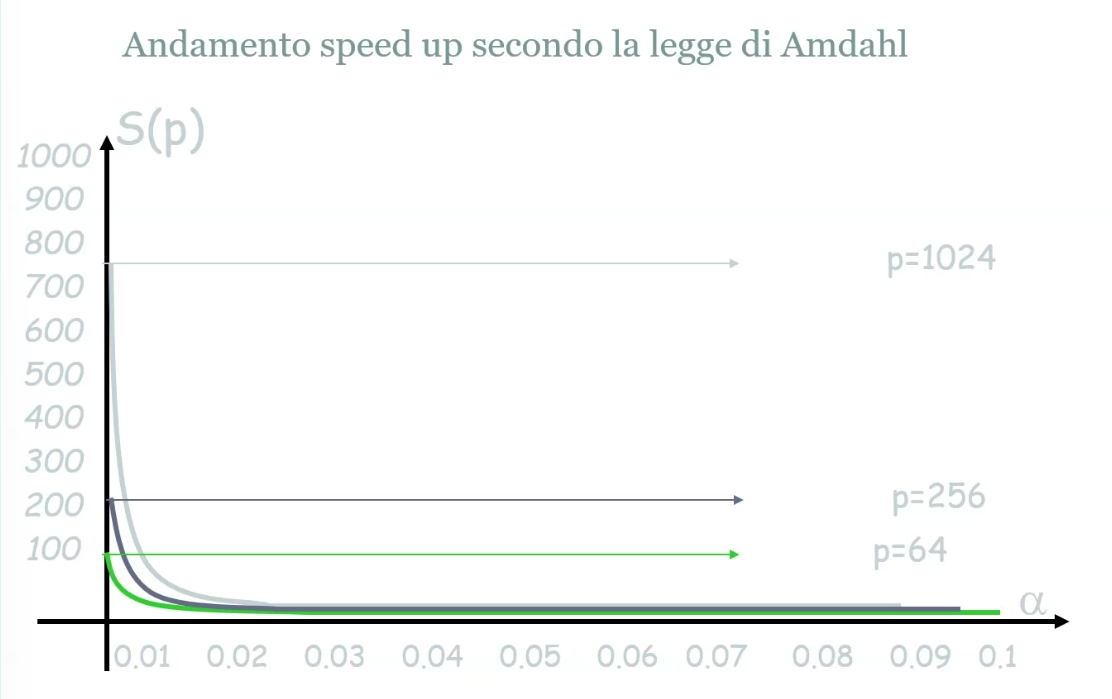
\includegraphics[width=0.5\textwidth]{../_files/_images/ware-amdahl.png}
\caption{Il valore dello speedup in funzione del parametro $\alpha$. Sono tracciati tre grafici: quello grigio chiaro ottenuto fissando $p=1024$, quello grigio scuro ottenuto fissando $p=256$, quello verde ottenuto fissando $p=1024$. Notiamo che per $\alpha > 0.01$, in tutti i tre grafici si osservano speed-up praticamente identici e molto bassi, nonostante il numero di processori sia molto diverso. Quindi, in ogni caso, una piccolissima crescita di $\alpha$ fa degradare $S(p)$.}
\label{fig:ware-amdahl}
\end{figure}

Consideriamo lo speedup come una funzione in due variabili $S(n;p)$. Se $p$ è fissato e $n$ cresce, si osserva $\alpha\to 0$ e quindi $S(p)\to p$. Se $n$ è fissato e $p$ cresce, si osserva una crescita di $S(n;p)$ fino ad un punto $n_{0}$ a partire dal quale la funzione si stabilizza (e quindi l'efficienza inizia a degradare).

\subsubsection{Legge di Ware-Amdahl generalizzata}
Si può rendere la legge di Ware-Amdahl più precisa definendo un rapporto $\alpha$ per ogni passo temporale dell'algoritmo in cui lavorano un certo numero di processori sui $p$ disponibili, ovvero
$$S(p) = \frac{1}{\alpha_1 + \frac{\alpha_2}{2} + ... + \frac{\alpha_p}{p}}$$
dove $\alpha_i$ corrisponde al rapporto $\frac{T_{c,i}}{T(1)}$, dove $T_{c,i}$ è il numero di operazioni eseguite da esattamente $i$ processori.

\begin{definition}{Scalabilità forte}
  Un algoritmo si dice **fortemente scalabile** se, fissata la dimensione del problema, l'efficienza rimane costante all'aumentare del numero di processori. 
\end{definition}

\subsubsection{Speedup scalato}
Denotiamo con $T(p,n)$ il tempo impiegato per risolvere un problema di dimensione $n$ con $p$ processori. Notiamo, per la seconda strategia della somma di $n$ numeri, che: 
\begin{itemize}
  \item se fissiamo $p$ e aumentiamo $n$, il valore di $\alpha$ scende fino a convergere a $0$, per cui lo speedup raggiunge il valore ideale;
  \item se fissiamo $n$ e aumentiamo $p$, si osserva il degrado dello speedup a partire da un certo $p_{0}$.
\end{itemize}
Invece, aumentando contemporaneamente il valore di $p$ e $n$, si osserva un aumento dello speedup ed una lenta discesa dell'efficienza, che quindi non degrada.
Ci aspettiamo che il tempo impiegato per risolvere un problema di dimensione $n$ con un solo processore sia uguale al tempo impiegato a risolvere un problema di dimensione $n\cdot p$ con $p$ processori, ovvero
$$T(1,n)=T(p, np)$$

Al variare congiunto di $n$ e $p$, estendiamo il concetto di speedup con quello di speedup scalato.

\begin{definition}{Speedup scalato}
Si definisce \keyword{speedup scalato} la quantità
$$SS(p,n) := \frac{T(1,np)}{T(p,np)} =\frac{pT(1,n)}{T(p,np)}$$
dove si assume che $T(1,np) = pT(1,n)$. 
\end{definition}

Analogamente, definiamo l'efficienza scalata.

\begin{definition}{Efficienza scalata}
Si definisce **efficienza scalata** la quantità
$$ES(p,n) := \frac{SS(p,n)}{p} = \frac{T(1,n)}{T(p,np)}$$
\end{definition}

\subsubsection{Legge di Gustafson}
Con lo stesso ragionamento che porta alla legge di Ware-Amdahl, consideriamo $$T(p) = T_s + T_c^{'}$$
con $T_c^{'} = \frac{T_c}{p}$, ovvero il numero di operazioni eseguite in parallelo da $p$ processori.

Ponendo il tempo $T(p)$ unitario, si ottiene 
$$T(p) = T_s + T_c^{'} = 1 \iff T_c^{'} = 1 - T_s$$
e quindi $T(1) = T_s + p(1-T_s)$. Infine, ponendo $T_s = \alpha^{'}$, si ottiene la **legge di Gustafson**:
$$SS(p) = \frac{T(1)}{T(p)} = \frac{\alpha^{'} + p(1-\alpha^{'})}{1} = p+(1-p)\alpha^{'}$$
A differenza della legge di Ware-Amdahl, che considerava la dimensione del problema come un parametro fissato, la legge di Gustafson ci dice che lo speedup scalato di un algoritmo si avvicina al valore perfetto, $p$, quando $\alpha'$ si avvicina a $0$ e ciò avviene al crescere delle operazioni totali, di cui si assume che solo una parte minore sia non parallelizzabile.

\begin{definition}{Scalabilità debole}
Un algoritmo si dice \keyword{debolmente scalabile} se la sua efficienza rimane costante all'aumentare congiunto di $n$ e $p$.
\end{definition}

\subsubsection{Isoefficienza}
L'\keyword{isoefficienza} è un'equazione che permette di calcolare come mantenere costante l'efficienza di un algoritmo. In altre parole, a partire da $n_{0}$ e $p_{0}$, come aumentare $n_{1}$ per mantenere invariata l'efficienza con $p_{1}$ processori?

$$\begin{aligned}
E(p_{0},n_{0})&=E(p_{1},n_{1}), \\
\frac{1}{\frac{O_{h}(n_{0},p_{0})}{T(1,n_{0})} + 1} &= \frac{1}{\frac{O_{h}(n_{1},p_{1})}{T(1,n_{1})} + 1}, \\
\frac{O_{h}(n_{0},p_{0})}{T(1,n_{0})} &= \frac{O_{h}(n_{1},p_{1})}{T(1,n_{1})}
\end{aligned}$$

\subsubsection{Tempo di comunicazione}
Consideriamo, adesso, il costo non trascurabile della comunicazione tra i processori. Il tempo per effettuare una singola comunicazione è denotato con $t_{\text{com}}$. In media, si osserva $\frac{1 t_{com}}{1 t_{calc}} = 10^3$. Il tempo di esecuzione di un algoritmo parallelo va infatti calcolato come somma dei tempi di calcolo e dei tempi di comunicazione, ovvero
$$T^{\text{time}}=T_{\text{com}}+T_{\text{calc}}$$
Si definisce \keyword{overhead di comunicazione} il rapporto
$$O_{c}(p) = \frac{T_{\text{com}}}{T_{\text{calc}}}$$

Come per le operazioni di calcolo, due comunicazioni che avvengono contemporaneamente valgono come una sola comunicazione, a livello di tempo di esecuzione dell'algoritmo parallelo.

Notiamo che, per $T_{\text{calc}}$ che cresce all'infinito, si osserva $O_{c}$ tendere a $0$, suggerendo che l'overhead di comunicazione sia molto pesante soprattutto per problemi di piccola dimensione. Infatti, nella somma di $n$ numeri, con $n$ piccolo e con una macchina MIMD Distributed Memory, la maggior parte del tempo di esecuzione è dovuto al message passing.
